\documentclass{beamer} % "Beamer" is a word used in Germany to mean video projector. 

\usetheme{Berkeley} % Search online for beamer themes to find your favorite or use the Berkeley theme as in this file.
\usepackage[slovene]{babel}
\usepackage[cp1250]{inputenc}
\usepackage{color} % It may be necessary to set PCTeX or whatever program you are using to output a .pdf instead of a .dvi file in order to see color on your screen.
\usepackage{graphicx} % This package is needed if you wish to include external image files.

\usepackage{amsmath,amssymb,amsfonts}
\usepackage{url}
\usepackage{authblk}

\theoremstyle{definition} % See Lesson Three of the LaTeX Manual for more on this kind of "proclamation."
\newtheorem*{dfn}{A Reasonable Definition}               

\title{Skriti markovski modeli v �asovnih vrstah}
%\newcommand{\imeavtorja}{Martin Pra�ek} % ime avtorja
%\newcommand{\imementorja}{izr. prof. dr. Damjan �kulj}
\institute{Fakulteta za matematiko in fiziko, Univerza v Ljubljani}
%\date{January 6, 2012} 
% Remove the % from the previous line and change the date if you want a particular date to be displayed; otherwise, today's date is displayed by default.

%\AtBeginSection[]  % The commands within the following {} will be executed at the start of each section.
%{%
%\begin{frame} % Within each "frame" there will be one or more "slides."  
%\frametitle{} % This is the title of the outline.
%\tableofcontents[currentsection]  % This will display the table of contents and highlight the current section.
%\end{frame}
%} % Do not include the preceding set of commands if you prefer not to have a recurring outline displayed during your presentation.

\begin{document}
\begin{frame}
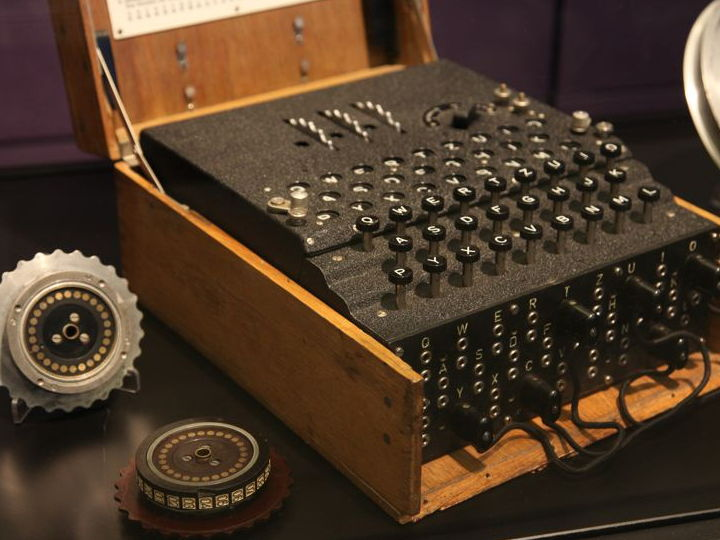
\includegraphics[width=.3\linewidth]{slike/enigma}\quad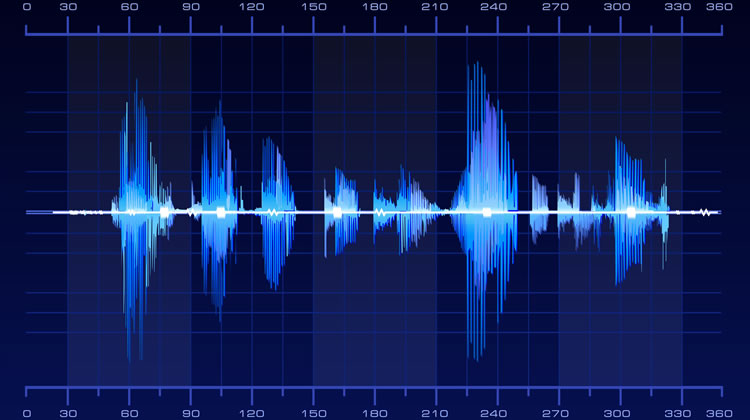
\includegraphics[width=.3\linewidth]{slike/govor}\quad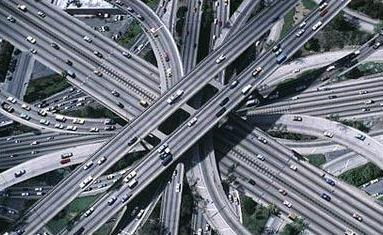
\includegraphics[width=.3\linewidth]{slike/transport}
\\[\baselineskip]% adds vertical line spacing

\includegraphics[width=.3\linewidth]{slike/lastnorocna}\quad
\includegraphics[width=.3\linewidth]{slike/gen}\quad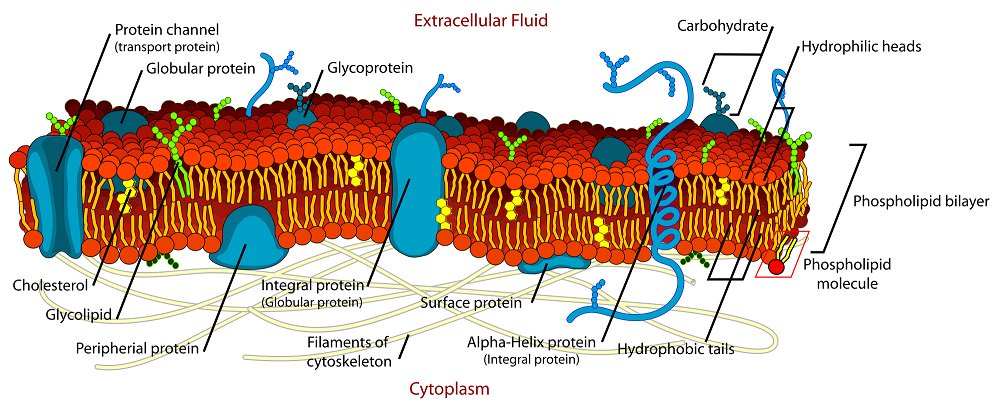
\includegraphics[width=.3\linewidth]{slike/celica1}
\end{frame}	

\begin{frame} 
\begin{titlepage}
	\begin{center}
		\vspace*{1cm}
		Martin Pra�ek \\
		Mentor: izr. prof. dr. Damjan �kulj
		
		\vspace{3cm}
		
\includegraphics[scale=1]{slike/logo}
		
		
		\vfill
		
		\large Ljubljana, december 2018
		
	\end{center}
\end{titlepage}
\end{frame}

\section{Markovski model} % Since this is the start of a new section, our recurring outline will appear here.

\begin{frame} 
\frametitle{Markovski model}
\begin{itemize}
	\item Markovska lastnost je lastnost slu�ajnega procesa, da je njegova vrednost v �asu $t$ odvisna le od njegove vrednosti v �asu $t-1$.
	\item Lo�imo v celoti opazovan in delno opazovan ter
	\item Avtonomen in kotroliran sistem.
\end{itemize}
\includegraphics[scale=0.5]{slike/veriga}
\end{frame}


\begin{frame}
\frametitle{Delitev markovskih modelov}
\includegraphics[width=10cm]{slike/slika1.png}
\end{frame}

\section{Skriti markovski model}
\begin{frame}
\frametitle{Skriti markovski model}
Skriti markovski model je statisti�ni markovski model, kjer predpostavljamo, da je modelirani sistem markovski proces z skritimi stanji.\\
Gre torej za tip modela, kjer lahko razberemo rezultat, ne moremo pa ugotoviti, kak�na je bila funkcija, ki nam ga je dala. 
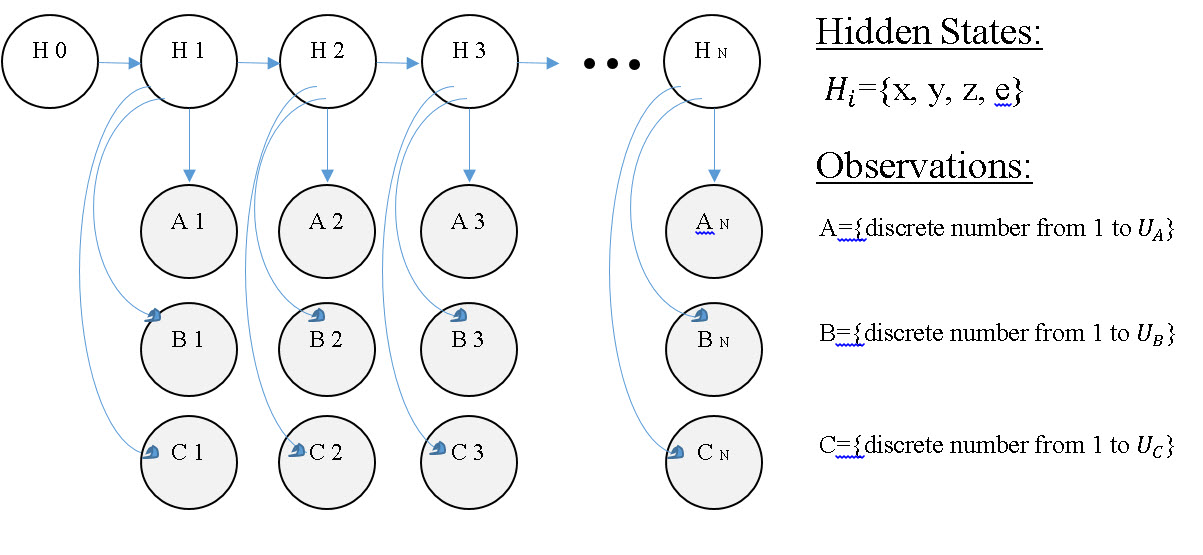
\includegraphics[scale=0.25]{slike/hmm} 
\end{frame}

\begin{frame}
\frametitle{Zahteve}
\begin{itemize}
	\item Markovska lastnost
	\item Enaki razdeljeni �asi signalov
	\item Sistem ima $N$ stanj, vsako dolo�a slu�ajna spremenjivka $S$
\end{itemize}
\includegraphics[scale=0.5]{slike/hmm2}
\end{frame}

\begin{frame}
\begin{itemize}
	\item Slu�ajnih spremenljivk v nobenem �asu ne poznamo, poznamo pa slu�ajni proces $Q$, ki predstavlja signale
	\item Vektor za�etnih stanj je $\Pi$
	\item Prehodna matrika $A$, ki je neodvisna od �asa
\end{itemize}
\end{frame}

\begin{frame}
\begin{itemize}
	\item Gaussove me�anice
	\item  $b_{i} = \sum_{j = 1}^{M}{c_{ij}} N(x;\mu_{j}, \sigma_{j}^2)$
	\item �tevilo me�anic $M$
	\item Matrike $\Gamma$, $\mu_{ij}$ predstavlja pri�akovano vrednost me�anice $j$ v stanju $i$
	\item $\Sigma$, kjer $\sigma_{ij}$ predstavlja varianco me�anice $j$ v stanju $i$
	\item $C$, koeficienti $c_{ij}$ iz Gaussove me�anice
\end{itemize}
\end{frame}

\begin{frame}
\frametitle{Osnovanje modela}
Da bomo lahko delali z na�im modelom, moramo najprej izvesti t.i. trening modela.
\begin{itemize}
	\item �op $k$-povpre�ij
	\item Akaikov informacijski kriterij
\end{itemize}
\includegraphics[scale=0.35]{slike/delnica}
\end{frame}

\begin{frame}
\frametitle{}
\end{frame}


\begin{frame}
\frametitle{Uporaba}
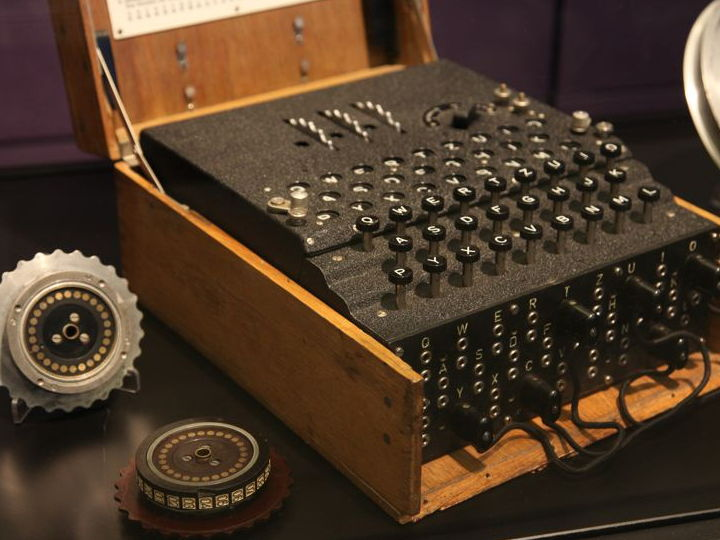
\includegraphics[width=.3\linewidth]{slike/enigma}\quad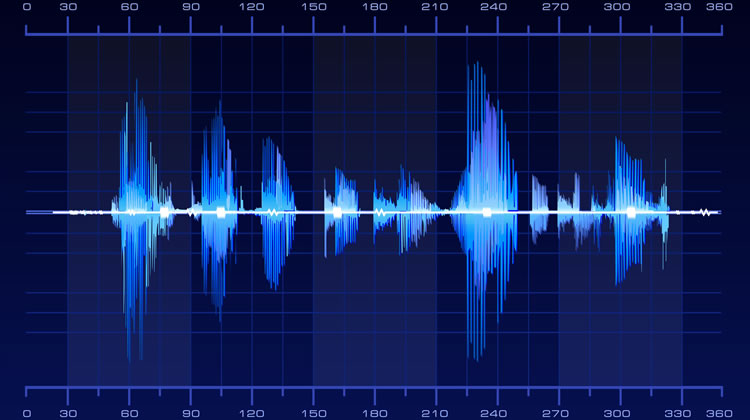
\includegraphics[width=.3\linewidth]{slike/govor}\quad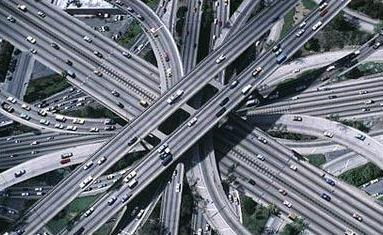
\includegraphics[width=.3\linewidth]{slike/transport}
\\[\baselineskip]% adds vertical line spacing

\includegraphics[width=.3\linewidth]{slike/lastnorocna}\quad
\includegraphics[width=.3\linewidth]{slike/gen}\quad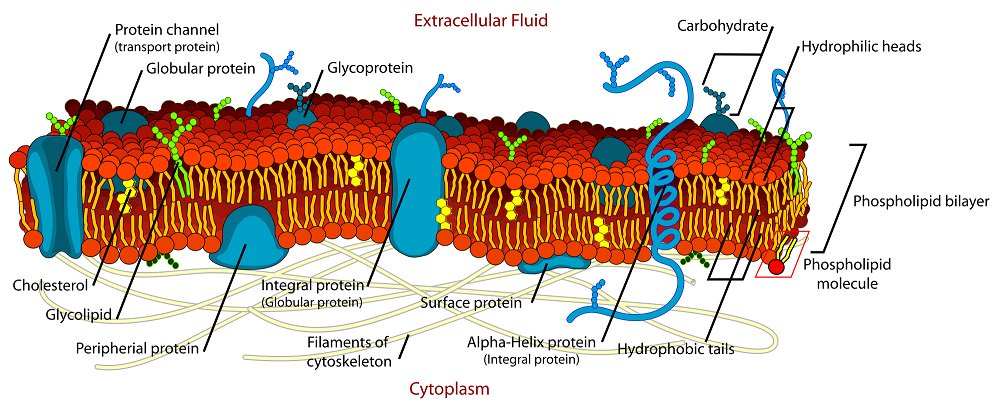
\includegraphics[width=.3\linewidth]{slike/celica1}
\end{frame}	

\section{Uporaba v �asovnih vrstah} % Since this is the start of a new section, our recurring outline will appear here.


\begin{frame}
\frametitle{}
\end{frame}

\begin{frame}
\frametitle{}
\end{frame}

\section{Kaj �e sledi?} % Since this is the start of a new section, our recurring outline will appear here.

\begin{frame}
V prihodnje bom tudi sam poizkusil dolo�iti skriti markovski model na svojem setu podatkov.

\end{frame}

\section{Viri}
\begin{frame}
\end{frame}


\end{document}

